\documentclass{article}
% Draw graph
\usepackage{tikz}
\usetikzlibrary{arrows.meta}
\usepackage{listings}
\usetikzlibrary{positioning, shapes.geometric}
% Set page size and margins
\usepackage[a4paper,top=2cm,bottom=2cm,left=3cm,right=3cm,marginparwidth=1.75cm]{geometry}

% Configure listings for code
\lstset{
    basicstyle=\ttfamily\small,           % Font style and size
    keywordstyle=\color{blue},            % Highlight keywords in blue
    commentstyle=\color{gray},            % Highlight comments in gray
    stringstyle=\color{red},              % Highlight strings in red
    numbers=left,                         % Line numbers on the left
    numberstyle=\tiny\color{gray},        % Line number font and color
    frame=single,                         % Add a frame around the code
    backgroundcolor=\color{lightgray},    % Set background color to light gray
    breaklines=true,                      % Enable line breaking
    captionpos=b                          % Place caption below the code
}

\title{Distributed System - Practical 1}
\author {Do Bao Nhi - 22BI13349}
\begin{document}
\maketitle

% Add table of contents, list of figures, and list of tables
\tableofcontents
\listoffigures
\clearpage

\section{Design Protocol}

We create a socket (communication endpoint) using the \texttt{socket()} function for both the client and the server. This enables them to exchange data using IP addresses.

\subsection{Client Side}

\begin{itemize}
    \item The \texttt{SERVER\_IP} and \texttt{SERVER\_PORT} are defined as the target server's IP address and port number, respectively.
    \item The \texttt{connect()} function is then used to establish a connection between the client and the server.
    \begin{itemize}
        \item The \texttt{connect()} function sends a \textbf{SYN} packet to the server and waits for the server to send back a \textbf{SYN-ACK} packet.
        \item Once the \textbf{SYN-ACK} is received, the client sends an \textbf{ACK} packet to complete the connection establishment process.
    \end{itemize}
    \item Once the connection is established, the client transfers the file to the server using the \texttt{send()} function.
    \item The client reads data from the file in chunks and sends it over the established connection.
    \item Finally, the \texttt{close()} function is used to terminate the communication.
\end{itemize}

\subsection{Server Side}

\begin{itemize}
    \item The \texttt{PORT} number is defined on which the server will listen for incoming requests.
    \item The \texttt{listen()} function is used to transition the server socket to passive mode, enabling it to wait for connection requests sent by the client (via \texttt{connect()}).
    \item When the server receives a \textbf{SYN} packet from the client:
    \begin{itemize}
        \item The server's TCP stack automatically sends a \textbf{SYN-ACK} packet back to the client.
        \item The server transitions to the \textbf{SYN\_RECEIVED} state while waiting for the client's \textbf{ACK} response.
    \end{itemize}
    \item Once the client sends the \textbf{ACK}, the connection is established.
    \item The \texttt{accept()} function is called to return a new socket dedicated to the established connection.
    \item At this point, the client and server can exchange data.
    \item The server uses the \texttt{recv()} function to receive data sent by the client.
    \item The received data is then written to a file using the \texttt{fprintf()} function.
    \item After all the data has been written to the file, the server socket is closed using the \texttt{close()} function.
\end{itemize}
\begin{figure}[h]
    \centering
    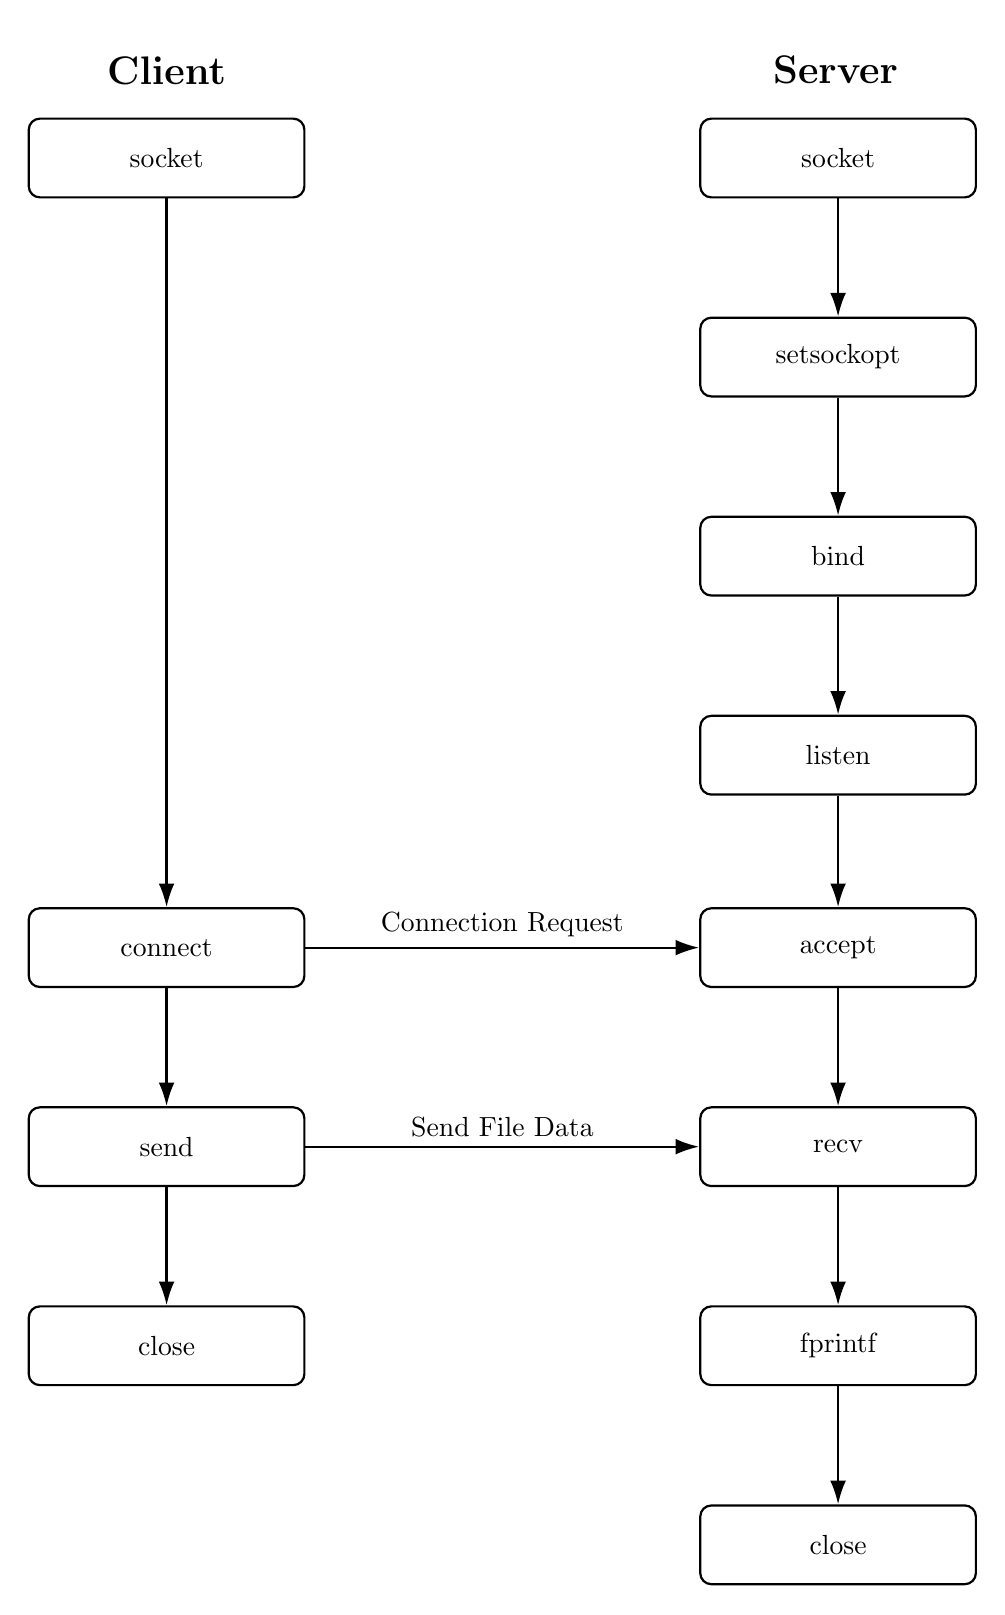
\begin{tikzpicture}[
            node distance=1.5cm and 2.5cm,
            protocol/.style={rectangle, draw=black, thick, rounded corners, minimum height=1cm, minimum width=3.5cm, align=center},
            arrow/.style={-{Latex[length=3mm, width=2mm]}, thick},
            column_line/.style={thick, dashed, gray},
            flow_arrow/.style={-{Latex[length=3mm, width=2mm]}, thick, black}
        ]
        
        % Labels for Client and Server
        \node[label, font=\Large\bfseries] (client_label) {Client};
        \node[label, right=6.7cm of client_label, font=\Large\bfseries] (server_label) {Server};
        
        % Columns (Client and Server)
        \node[protocol, below=0.3cm of client_label] (client_socket) {socket};
        \node[protocol, below=9cm of client_socket] (client_connect) {connect}; % Explicitly position connect
        \node[protocol, below=of client_connect] (client_send) {send};
        \node[protocol, below=of client_send] (client_close) {close};
        
        \node[protocol, right=5cm of client_socket] (server_socket) {socket};
        \node[protocol, below=of server_socket] (server_setsockopt) {setsockopt};
        \node[protocol, below=of server_setsockopt] (server_bind) {bind};
        \node[protocol, below=of server_bind] (server_listen) {listen};
        \node[protocol, right=5cm of client_connect] (server_accept) {accept}; % Align accept with connect
        \node[protocol, below=of server_accept] (server_read) {recv};
        \node[protocol, below=of server_read] (server_write) {fprintf};
        \node[protocol, below=of server_write] (server_close) {close};
        
        % Vertical lines (columns)
        \draw[column_line, opacity=0] (client_socket.north) -- (client_close.south);
        \draw[column_line, opacity=0] (server_socket.north) -- (server_close.south);
        
        % Vertical arrows (Client)
        \draw[flow_arrow] (client_socket.south) -- (client_connect.north);
        \draw[flow_arrow] (client_connect.south) -- (client_send.north);
        \draw[flow_arrow] (client_send.south) -- (client_close.north);
        
        % Vertical arrows (Server)
        \draw[flow_arrow] (server_socket.south) -- (server_setsockopt.north);
        \draw[flow_arrow] (server_setsockopt.south) -- (server_bind.north);
        \draw[flow_arrow] (server_bind.south) -- (server_listen.north);
        \draw[flow_arrow] (server_listen.south) -- (server_accept.north);
        \draw[flow_arrow] (server_accept.south) -- (server_read.north);
        \draw[flow_arrow] (server_read.south) -- (server_write.north);
        \draw[flow_arrow] (server_write.south) -- (server_close.north);
        
        % Arrows between Client and Server
        \draw[arrow] (client_connect.east) -- node[midway, above] {Connection Request} (server_accept.west);
        \draw[arrow] (client_send.east) -- node[midway, above] {Send File Data} (server_read.west);
        
    
    \end{tikzpicture}
    \caption{Client-Server Interaction Protocol}
\end{figure}

\clearpage
\section{System Architecture}

The system consists of a server and a client, which communicate with each other using a stream socket. A stream socket allows processes to utilize the \textbf{Transmission Control Protocol (TCP)} for communication. Since TCP is a connection-oriented protocol, it requires a connection to be established before data can be transferred. The responsibilities of each component are as follows:

\subsection*{Client}
\begin{itemize}
    \item Sends a \textbf{SYN} request to initiate the connection.
    \item Receives a \textbf{SYN-ACK} response from the server and then sends an \textbf{ACK} to complete the handshake.
    \item Once the connection is established, the client sends a file to the server.
\end{itemize}

\subsection*{Server}
\begin{itemize}
    \item Listens for incoming connection requests.
    \item Receives the \textbf{SYN} request from the client and responds with a \textbf{SYN-ACK} packet.
    \item Receives the client's \textbf{ACK} to complete the connection establishment.
    \item After the connection is established, the server receives the file from the client and writes the data to a file.
\end{itemize}

\begin{figure}[h]
    \centering
    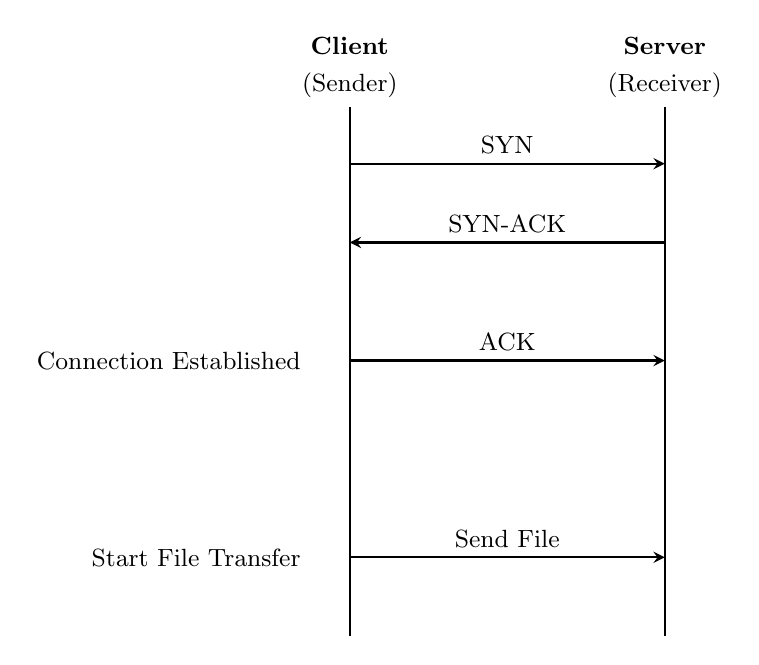
\begin{tikzpicture}[
        node distance=1.5cm and 2.5cm,
        on grid,
        >=stealth,
        every node/.style={font=\small}
    ]

    % Nodes for Client and Server
    \node[align=center] (client) {(Sender)};
    \node[align=center,right=4cm of client] (server) {(Receiver)};

    % Vertical lines
    \draw[thick] (client) -- ++(0,-7) coordinate (CLine);
    \draw[thick] (server) -- ++(0,-7) coordinate (SLine);

    % Add titles for Client and Server
    \node[above=0.5cm of client] {\textbf{Client}};
    \node[above=0.5cm of server] {\textbf{Server}};

    % SYN Arrow
    \draw[->,thick] (client) ++(0,-1) coordinate (SYNStart)
        -- ++(4,0) node[midway, above] {SYN};

    % SYN-ACK Arrow
    \draw[->,thick] (server) ++(0,-2) coordinate (SYNACKStart)
        -- ++(-4,0) node[midway, above] {SYN-ACK};

    % ACK Arrow
    \draw[->,thick] (client) ++(0,-3.5) coordinate (ACKStart)
        -- ++(4,0) node[midway, above] {ACK};

    % Label for Connection Established
    \node[left=0.5cm] at (client.south |- ACKStart) {Connection Established};

    % File Transfer Arrow (Client -> Server)
    \draw[->,thick] (client) ++(0,-6) coordinate (FileSendStart)
        -- ++(4,0) node[midway, above] {Send File};

    % Labels for File Transfer Process
    \node[left=0.5cm] at (client.south |- FileSendStart) {Start File Transfer};

    \end{tikzpicture}
    \caption{TCP Handshake and File Transfer Process}
\end{figure}

\clearpage
\section{Implementation}
\subsection{send\_file() Function in the client side}

The \texttt{send\_file()} function is responsible for sending a file from the client to the server. It reads the file in chunks and transmits each chunk to the server over an established socket connection.

\begin{lstlisting}[language=C, caption={send\_file() Function in the Client Side}, label={lst:send_file}]
void send_file(FILE *fp, int client_socket) {
    int n;
    char buffer[BUFFER_SIZE];
    while(fgets(buffer, BUFFER_SIZE, fp) != NULL) {
        if(send(client_socket, buffer, sizeof(buffer), 0) == -1) {
            perror("[-] Sending file failed");
            exit(EXIT_FAILURE);
        }
        bzero(buffer, BUFFER_SIZE);
    }
}
\end{lstlisting}

\subsection{recv\_file() Function in the server side}

The \texttt{recv\_file()} function is responsible for receiving a file sent by the client. It reads data from the client socket in chunks, writes the received data into a file, and continues until the connection is closed or an error occurs.

\begin{lstlisting}[language=C, caption={recv\_file() Function in the Server Side}, label={lst:recv_file}]
void recv_file(int client_socket) {
    int n;
    FILE *fp;
    char *fn = "message.txt";
    char buffer[BUFFER_SIZE];

    fp = fopen(fn, "w");
    // Loop until the connection is closed or an error occurs
    while (1) {
        // recv() returns the number of bytes read
        n = recv(client_socket, buffer, BUFFER_SIZE, 0);
        if (n <= 0) {
            break;
        }
        // Write the received data to message.txt
        fprintf(fp, "%s", buffer);
        bzero(buffer, BUFFER_SIZE); // Clear all data in the buffer
    }
    fclose(fp);
}
\end{lstlisting}

\subsection{Result}

\subsubsection{Client output}
The following image shows the client-side output captured during the execution of the program
\begin{figure}[h]
    \centering
    \includegraphics[width=0.8\textwidth]{image_c.png} 
    \caption{Client-side output.}
    \label{fig:client_output}
\end{figure}

\clearpage
\subsubsection{Server output}
The following image shows the server-side output captured during the execution of the program.

\begin{figure}[h!]
    \centering
    \includegraphics[width=0.8\textwidth]{image_s.png} 
    \caption{Server-side output.}
    \label{fig:server_output}
\end{figure}

\noindent
This image indicates that the client send the \textbf{send.txt }file to the server over connection. Then server received the file data from client and write these data to \textbf{message.txt} file.

\begin{figure}[h]
    \centering
    \includegraphics[width=0.8\textwidth]{image.png} 
    \caption{File data transferred.}
    \label{fig:file}
\end{figure}

\end{document}
